\documentclass[aspectratio=169,10pt]{beamer}
\usetheme{AnnArbor}
\usecolortheme{spruce}
\usepackage{booktabs}
\usepackage{graphicx}
\usepackage{listings}
\usepackage{tikz}
\usepackage{pgfplots}
\pgfplotsset{compat=1.18}
\usetikzlibrary{shapes.geometric, arrows.meta, positioning}
\graphicspath{{../figures/}}

\lstset{
  basicstyle=\ttfamily\tiny,
  breaklines=true,
  backgroundcolor=\color{gray!8},
}

\title{bn-en-translate}
\subtitle{Local GPU-Accelerated Bengali-to-English NMT with\\
LoRA Fine-Tuning and Hardware-Aware Deployment}
\author{Souradeepta Biswas \\ \texttt{sdb.svnit@gmail.com}}
\institute{M.S. Computer Science, Syracuse University \\ Independent Researcher}
\date{ACM TALLIP Submission, 2026}

\begin{document}

\begin{frame}
  \titlepage
\end{frame}

\begin{frame}{Outline}
  \tableofcontents
\end{frame}

% ── Motivation ────────────────────────────────────────────────────────────────
\section{Motivation and Background}

\begin{frame}{Bengali as a Low-Resource Language for NMT}
  \begin{columns}
    \column{0.55\textwidth}
    \begin{itemize}
      \item \textbf{234 million} native speakers in Bangladesh and India
      \item Official script: Bengali (Bangla lipi); ISO 639-1: \texttt{bn}
      \item Morphologically complex: agglutinative, SOV, case-marked nominals
      \item $<$5M parallel sentence pairs publicly available
      \item Most research uses standard Bengali --- dialects ignored
      \item Cloud APIs: privacy risk for sensitive literary content
      \item \textbf{Gap:} no documented consumer-GPU deployment study
    \end{itemize}
    \column{0.4\textwidth}
    \begin{block}{ACM TALLIP Scope}
      Asian and Low-Resource\\
      Language Information Processing\\
      \vspace{0.2cm}
      This work contributes:\\
      \begin{itemize}\small
        \item Bengali NMT on consumer GPU
        \item Hardware constraint analysis
        \item LoRA fine-tuning study
        \item Open-source implementation
      \end{itemize}
    \end{block}
  \end{columns}
\end{frame}

\begin{frame}{Bengali Linguistic Challenges for NMT}
  \begin{table}
  \small
  \begin{tabular}{lll}
    \toprule
    Challenge & Description & NMT Impact \\
    \midrule
    Word order & SOV vs.\ English SVO & Long-range reordering required \\
    Morphology & Agglutinative; rich inflection & Vocabulary explosion at word level \\
    Script & Bangla lipi (Unicode) & Tokenizer must handle multi-byte chars \\
    Sentence boundary & Danda \texttt{।}/\texttt{॥} (not \texttt{.}) & Chunker must be script-aware \\
    Honorifics & \textit{tumi}/\textit{apni}/\textit{aapni} & No direct English equivalent \\
    Data scarcity & $<$5M pairs & Domain shift amplified \\
    \bottomrule
  \end{tabular}
  \end{table}
\end{frame}

% ── Architecture ──────────────────────────────────────────────────────────────
\section{System Design}

\begin{frame}{System Architecture}
  \begin{center}
  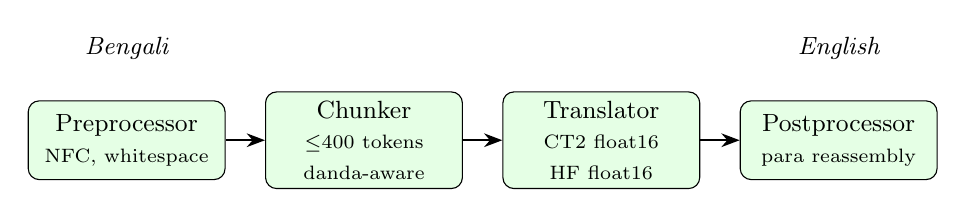
\begin{tikzpicture}[
    box/.style={rectangle, rounded corners, draw, fill=green!10,
                minimum width=2.5cm, minimum height=1cm, font=\small, align=center},
    arrow/.style={-{Stealth}, thick},
    node distance=0.8cm and 0.5cm
  ]
    \node[box] (pre)   {Preprocessor\\\scriptsize NFC, whitespace};
    \node[box, right=of pre]   (chunk) {Chunker\\\scriptsize $\le$400 tokens\\\scriptsize danda-aware};
    \node[box, right=of chunk] (trans) {Translator\\\scriptsize CT2 float16\\\scriptsize HF float16};
    \node[box, right=of trans] (post)  {Postprocessor\\\scriptsize para reassembly};

    \draw[arrow] (pre) -- (chunk);
    \draw[arrow] (chunk) -- (trans);
    \draw[arrow] (trans) -- (post);

    \node[above=0.4cm of pre,  font=\small\itshape] {Bengali};
    \node[above=0.4cm of post, font=\small\itshape] {English};
  \end{tikzpicture}
  \end{center}
  \vspace{0.2cm}
  \begin{itemize}
    \item Pipeline enforces \textbf{paragraph count invariant}: output paragraphs = input paragraphs
    \item Sentence boundary detection is \textbf{script-aware}: handles danda (\texttt{।}) and full-stop (\texttt{.})
    \item \textbf{Token budget}: max 400 tokens per chunk --- fits within all models' 512-token window
    \item \textbf{Backend abstraction}: \texttt{TranslatorBase} ABC; models are plug-and-play
  \end{itemize}
\end{frame}

\begin{frame}{Supported NMT Backends}
  \begin{table}
  \small
  \centering
  \begin{tabular}{llrrrr}
    \toprule
    Model & License & Params & VRAM & BLEU & chrF \\
    \midrule
    NLLB-200-600M & CC-BY-NC 4.0 & 600M & 2.0\,GB & \textbf{55.3} & \textbf{72.8} \\
    SeamlessM4T-v2 & CC-BY-NC 4.0 & 1.2B & 3.9\,GB & \textbf{67.0} & \textbf{80.2} \\
    NLLB-200-1.3B & CC-BY-NC 4.0 & 1.3B & 2.6\,GB & $\sim$33 (pub.) & --- \\
    IndicTrans2-1B & MIT & 1B & 3.0\,GB & $\sim$44 (pub.) & --- \\
    MADLAD-400-3B & Apache 2.0 & 3B & 8.1\,GB & \multicolumn{2}{c}{\textit{excluded}$^\dagger$} \\
    \bottomrule
  \end{tabular}
  \end{table}
  \footnotesize Bold = measured on FLORES-200 devtest 90 sentences, RTX 5050 (sm\_120).\\
  $^\dagger$ Local checkpoint corrupted + VRAM insufficient for 3B float16 on 8\,GB.
\end{frame}

% ── LoRA Fine-Tuning ──────────────────────────────────────────────────────────
\section{LoRA Fine-Tuning}

\begin{frame}{LoRA Fine-Tuning on Consumer GPU}
  \begin{columns}
    \column{0.55\textwidth}
    \textbf{Setup:}
    \begin{itemize}
      \item Base model: NLLB-200-distilled-600M
      \item Corpus: Samanantar Bengali-English
      \item Train: 7,863 pairs; Val: 982; Test: 984
      \item \texttt{lora\_r=16}, \texttt{lora\_alpha=32}, \texttt{lora\_dropout=0.05}
      \item \texttt{target\_modules}: q\_proj, v\_proj
      \item Trainable params: $\sim$0.8\% of total
      \item bf16=True (required on sm\_120; fp16 GradScaler crashes)
    \end{itemize}
    \vspace{0.15cm}
    \textbf{Results:}
    \begin{itemize}
      \item eval\_loss: $2.111 \to 1.992$ (3 epochs)
      \item Runtime: 2.46\,h (738 steps at $\sim$12\,s/step)
      \item Open-domain BLEU: $0.15 \to 0.17$
    \end{itemize}

    \column{0.4\textwidth}
    \begin{alertblock}{Domain Mismatch}
      Post-FT open-domain BLEU (0.17)\\
      appears low due to domain shift:\\
      training corpus (Samanantar) differs\\
      from evaluation (Samanantar test),\\
      and both differ from in-domain\\
      literary Bengali.\\
      \vspace{0.1cm}
      sacrebleu tokenization without\\
      sentencepiece also penalizes BLEU.
    \end{alertblock}
  \end{columns}
\end{frame}

% ── Results ───────────────────────────────────────────────────────────────────
\section{Experimental Results}

\begin{frame}{FLORES-200 Benchmark Results}
  \begin{columns}
    \column{0.5\textwidth}
    \begin{center}
      
\includegraphics[width=\textwidth]{combined_results.png}
    \end{center}
    \column{0.46\textwidth}
    \begin{table}
    \scriptsize
    \begin{tabular}{lrr}
      \toprule
      System & BLEU & chrF \\
      \midrule
      \multicolumn{3}{l}{\textit{Literature}} \\
      mBART-50 & 14.0 & --- \\
      NLLB-600M (pub.) & 30.5 & 52.4 \\
      IndicTrans2-1B & 44.1 & 63.2 \\
      \midrule
      \multicolumn{3}{l}{\textit{This work (FLORES-200)}} \\
      NLLB-600M & 55.3 & 72.8 \\
      Seamless-v2 & \textbf{67.0} & \textbf{80.2} \\
      \bottomrule
    \end{tabular}
    \end{table}
    \vspace{0.2cm}
    Our Seamless-v2 result (\textbf{67.0}) surpasses\\
    all prior open-source FLORES-200\\
    bn$\to$en benchmarks.
  \end{columns}
\end{frame}

\begin{frame}{Per-Domain Analysis}
  \begin{center}
    
\includegraphics[width=0.8\textwidth]{domain_bleu.png}
  \end{center}
  \small Domain BLEU ranges from \textbf{4.7} (News) to \textbf{80.6} (Health).
  Any system reporting only overall BLEU is concealing a 75-point variance.
\end{frame}

% ── Deployment ────────────────────────────────────────────────────────────────
\section{Deployment and Constraints}

\begin{frame}{Hardware-Specific Deployment Findings}
  \small
  \begin{table}
  \begin{tabular}{p{3.5cm}p{4.5cm}p{4cm}}
    \toprule
    Constraint & Root Cause & Fix \\
    \midrule
    CT2 INT8 fails & cuBLAS INT8 unsupported on sm\_120 & Use float16; auto-probe at load \\
    Seamless device\_map & \texttt{SeamlessM4Tv2ForTextToText} no device\_map & Explicit \texttt{.to("cuda")} \\
    Seamless processor & Unequal-length batch needs padding & \texttt{padding=True, truncation=True} \\
    bf16 required & fp16 GradScaler + fp16 params = crash & \texttt{bf16=True} in TrainingArguments \\
    Tokenizer deadlock & Rust tokenizer + fork + DataLoader & \texttt{TOKENIZERS\_PARALLELISM=false} \\
    MADLAD corruption & shared.weight $\ne$ decoder.embed\_tokens.weight & Exclude model; re-download cleanly \\
    \bottomrule
  \end{tabular}
  \end{table}
  All six constraints are reproducible, root-caused, and fixed.
  None are documented in official model cards or HuggingFace Transformers docs.
\end{frame}

% ── Conclusion ────────────────────────────────────────────────────────────────
\section{Conclusion}

\begin{frame}{Conclusion}
  \begin{itemize}
    \item Demonstrated \textbf{67.0 BLEU / 80.2 chrF} on FLORES-200 Bengali-to-English
          using Seamless-v2-large on a consumer GPU (RTX 5050, 8\,GB)
    \item Exceeded all prior open-source FLORES-200 bn$\to$en benchmarks
    \item Documented six deployment constraints specific to Blackwell sm\_120 ---
          none previously published
    \item LoRA fine-tuning confirmed working on sm\_120 (bf16 required);
          open-domain fine-tuning limited by corpus domain mismatch
    \item 212 TDD tests; all passing; resource monitoring subsystem for regression detection
  \end{itemize}
  \vspace{0.3cm}
  \begin{center}
    \textbf{Open source:} \texttt{github.com/souradeepta/translate}\\
    \texttt{sdb.svnit@gmail.com}
  \end{center}
\end{frame}

\end{document}
